\documentclass[12pt]{article}
\usepackage{times}
\usepackage[english]{babel}
\usepackage[utf8x]{inputenc}
\usepackage[colorinlistoftodos]{todonotes}
\usepackage[margin=1in]{geometry}
\usepackage{graphicx}
\usepackage{epstopdf}
\usepackage{cite}
\usepackage{listings}
\usepackage{dtklogos}
\usepackage{wrapfig}
\usepackage{subfigure}
\usepackage{amsmath}
\usepackage{amsthm}
\usepackage{amssymb}
\usepackage{amscd}
\usepackage{caption}
\usepackage{etoolbox}
\usepackage{fancyhdr}
\usepackage{stackengine}
\usepackage[export]{adjustbox}
\patchcmd{\thebibliography}{\section*{\refname}}{}{}{}
\usepackage[document]{ragged2e}    %This causes text to left align
\usepackage[colorlinks=true, linkcolor=black,citecolor=black,urlcolor=blue]{hyperref}
\bibliographystyle{IEEEtran}
\DeclareGraphicsRule{.tif}{png}{.png}{`convert #1 `dirname #1`/`basename #1 .tif`.png}

\title{MCHE 474: Lab 1}

\begin{document}
\lefthyphenmin3
\righthyphenmin4
% \pretolerance=2000
% \tolerance=500 
% \emergencystretch=10pt
%\raggedright     %Stops LaTeX from automatically hyphenating the right margin to fit better
%Combine this with \usepackage[document]{ragged2e} to get a text align left similar to natural MS Word


%-------------------------------------------------------------
%Start of Paper
%-------------------------------------------------------------

%%%%%%%%%%%%%%%%%%%%%%%%%%%%%%%%%%%%%%%%%%%%%%%%%%%%%%
%%%%%%%%%%%%%%%%%%%%%%% TITLE PAGE %%%%%%%%%%%%%%%%%%%%%%%%
%%%%%%%%%%%%%%%%%%%%%%%%%%%%%%%%%%%%%%%%%%%%%%%%%%%%%%

\begin{titlepage}

\newcommand{\HRule}{\rule{\linewidth}{0.5mm}} % Defines a new command for the horizontal lines, change thickness here

\center % Center everything on the page
 
%----------------------------------------------------------------------------------------
%	Heading Section
%----------------------------------------------------------------------------------------

\textsc{\LARGE University of Louisiana at Lafayette}\\[1.5cm] % Name of your university/college
\textsc{\Large Control Systems}\\[0.5cm] % Major heading such as course name
\textsc{\large MCHE 474}\\[0.5cm] % Minor heading such as course title

%----------------------------------------------------------------------------------------
%	Title Section
%----------------------------------------------------------------------------------------

\HRule \\[0.4cm]
{ \huge \bfseries Lab 1}\\[0.4cm] % Title of your document
\HRule \\[1.5cm]
 
%----------------------------------------------------------------------------------------
%	Author Section
%----------------------------------------------------------------------------------------

\begin{minipage}{0.4\textwidth}
\begin{flushleft} \large
\emph{Author:}\\
\textsc{Matthew J. Begneaud} \\% Your name
\end{flushleft}
\end{minipage}
~
\begin{minipage}{0.4\textwidth}
\begin{flushright} \large
\emph{Professor:} \\
\textsc{Dr. Mostafa A. Elsayed} % Supervisor's Name
\end{flushright}
\end{minipage}\\[1.5cm]

% If you don't want a supervisor, uncomment the two lines below and remove the section above
%\Large \emph{Author:}\\
%John \textsc{Smith}\\[3cm] % Your name

%----------------------------------------------------------------------------------------
%	Date Section
%----------------------------------------------------------------------------------------

{\textsc{\large \today}}\\[2cm] % Date, change the \today to a set date if you want to be precise

%----------------------------------------------------------------------------------------
%	Logo Section
%----------------------------------------------------------------------------------------


\includegraphics[width=5in]{UL_logo.jpg}\\[1cm] % Include a department/university logo - this will require the graphicx package
 
%----------------------------------------------------------------------------------------

\vfill % Fill the rest of the page with whitespace

\end{titlepage}

%%%%%%%%%%%%%%%%%%%%%%%%%%%%%%%%%%%%%%%%%%%%%%%%%%%%%%
%%%%%%%%%%%%%%%%%%%%%%% TABLE OF CONTENTS %%%%%%%%%%%%%%%%%%%
%%%%%%%%%%%%%%%%%%%%%%%%%%%%%%%%%%%%%%%%%%%%%%%%%%%%%%

\large \tableofcontents

\large \bigskip

\large \listoffigures

\newpage

%%%%%%%%%%%%%%%%%%%%%%%%%%%%%%%%%%%%%%%%%%%%%%%%%%%%%%
%%%%%%%%%%%%%%%%%%%%%%% REPORT %%%%%%%%%%%%%%%%%%%%%%%%%%
%%%%%%%%%%%%%%%%%%%%%%%%%%%%%%%%%%%%%%%%%%%%%%%%%%%%%%

\addcontentsline{toc}{section}{Introduction} % Add before each section
\section*{\fontsize{12}{12}\selectfont \large Introduction}
This lab was conducted by utilizing MATLAB, specifically the Simulink package, in order to analyze control signal diagrams. These diagrams consisted of gains, summation points, transfer functions, and feedback loops. These systems were analyzed with the main goal of obtaining the time response. The systems to be analyzed are shown in Figure 1. 
\bigskip
\bigskip

% Figure 1
\begin{figure}[htbp] %  figure placement: here, top, bottom, or page
   \centering
   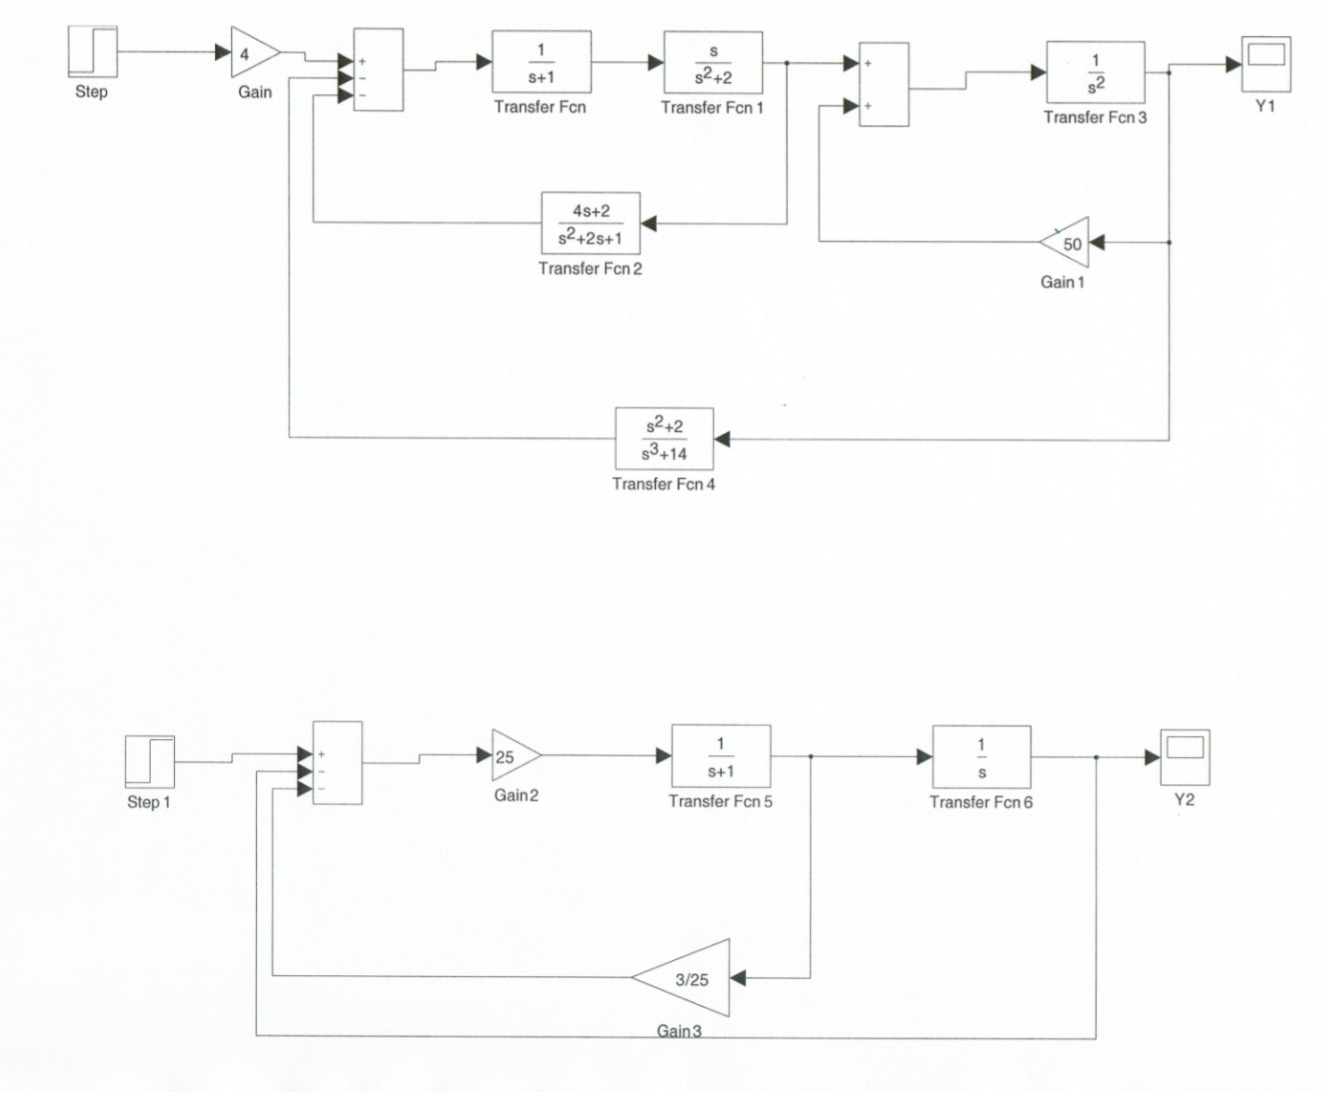
\includegraphics[width=\linewidth]{signal_diagrams.jpg} 
   \caption{Signal Diagrams}
   \label{fig:example}
\end{figure}

\newpage


\addcontentsline{toc}{section}{Theory} % Add before each section
\section*{\fontsize{12}{12}\selectfont \large Theory}
Signals in control systems are manipulated by various means. Passing a signal through a gain simply increases, or decreases, a signal strength, which is quite useful. Signals can also go through feedback loops. Feedback loops can make the system more robust. For example, passing a signal to an actuator without any sensing cannot provide any feedback as to what the outcome is. This is detrimental if the actuator is not receiving enough power in order to carry out its desired task, or if the actuator has reached a goal position and needs to stop. Having sensors gives the system feedback which can ensure the system performs as intended. Feedback loops can be negative or positive depending on the desired function of the loop. 
\bigskip

Signals are also commonly passed through transfer functions. A transfer function compares the output to the input of a linear system, time-variant systems. Transfer functions are in the frequency domain, which correlates to the Laplace domain. The time domain expression of the output is typically of interest in control systems, and using the transfer function of a system can help to obtain the time-response of the system. The general form of a transfer function for a system with input $R(s)$ and output $Y(s)$ is shown in Equations 1 and 2 as follows,
\bigskip

\begin{equation}
H(s) = \frac{Y(s)}{R(s)} 
\end{equation}
\begin{equation}
H(s) = \frac{L[y(t)]}{L[r(t)]}
\end{equation}
\bigskip

where $L$ is the Laplace transform operator and the time domain representations of the system input and output are $r(t)$ and $y(t)$, respectively.
\bigskip

Systems can also be described by their status as either stable or unstable. A stable system eventually approaches and tends to stay at some constant settling value known as a steady state value, as shown in Figure 2, until some external disturbance acts on it. Once that external disturbance is removed, the system returns to the steady state value. Unstable systems will not settle on their own and will continue to change even when there are no external disturbances acting on the system.
\bigskip

Systems also have other characteristics, such as overshoot. Overshoot is when the system output exceeds the steady state value, and can be seen in Figure 2 when the system output exceeds the step input at first. The overshoot is often described as a percentage, which can be calculated with Equation 3 as follows:
\bigskip

\begin{equation}
O.S. = \frac{Max Value - Steady State Value}{Steady State Value}*100
\end{equation}
\bigskip

Systems can also be described by rise time, which is defined as the time taken to rise from a low value state to a higher value state, and helps describe a system's ability to respond to sudden inputs. A system also has a characteristic settling time which is the time taken for the system to reach a state that lies within a specified range of error after responding to a step input. The system depicted in Figure 2 can be seen to reach a state which lies within a specified range of error after some time, for example.
\bigskip


% Figure 2
\begin{figure}[h!] %  figure placement: here, top, bottom, or page
   \centering
   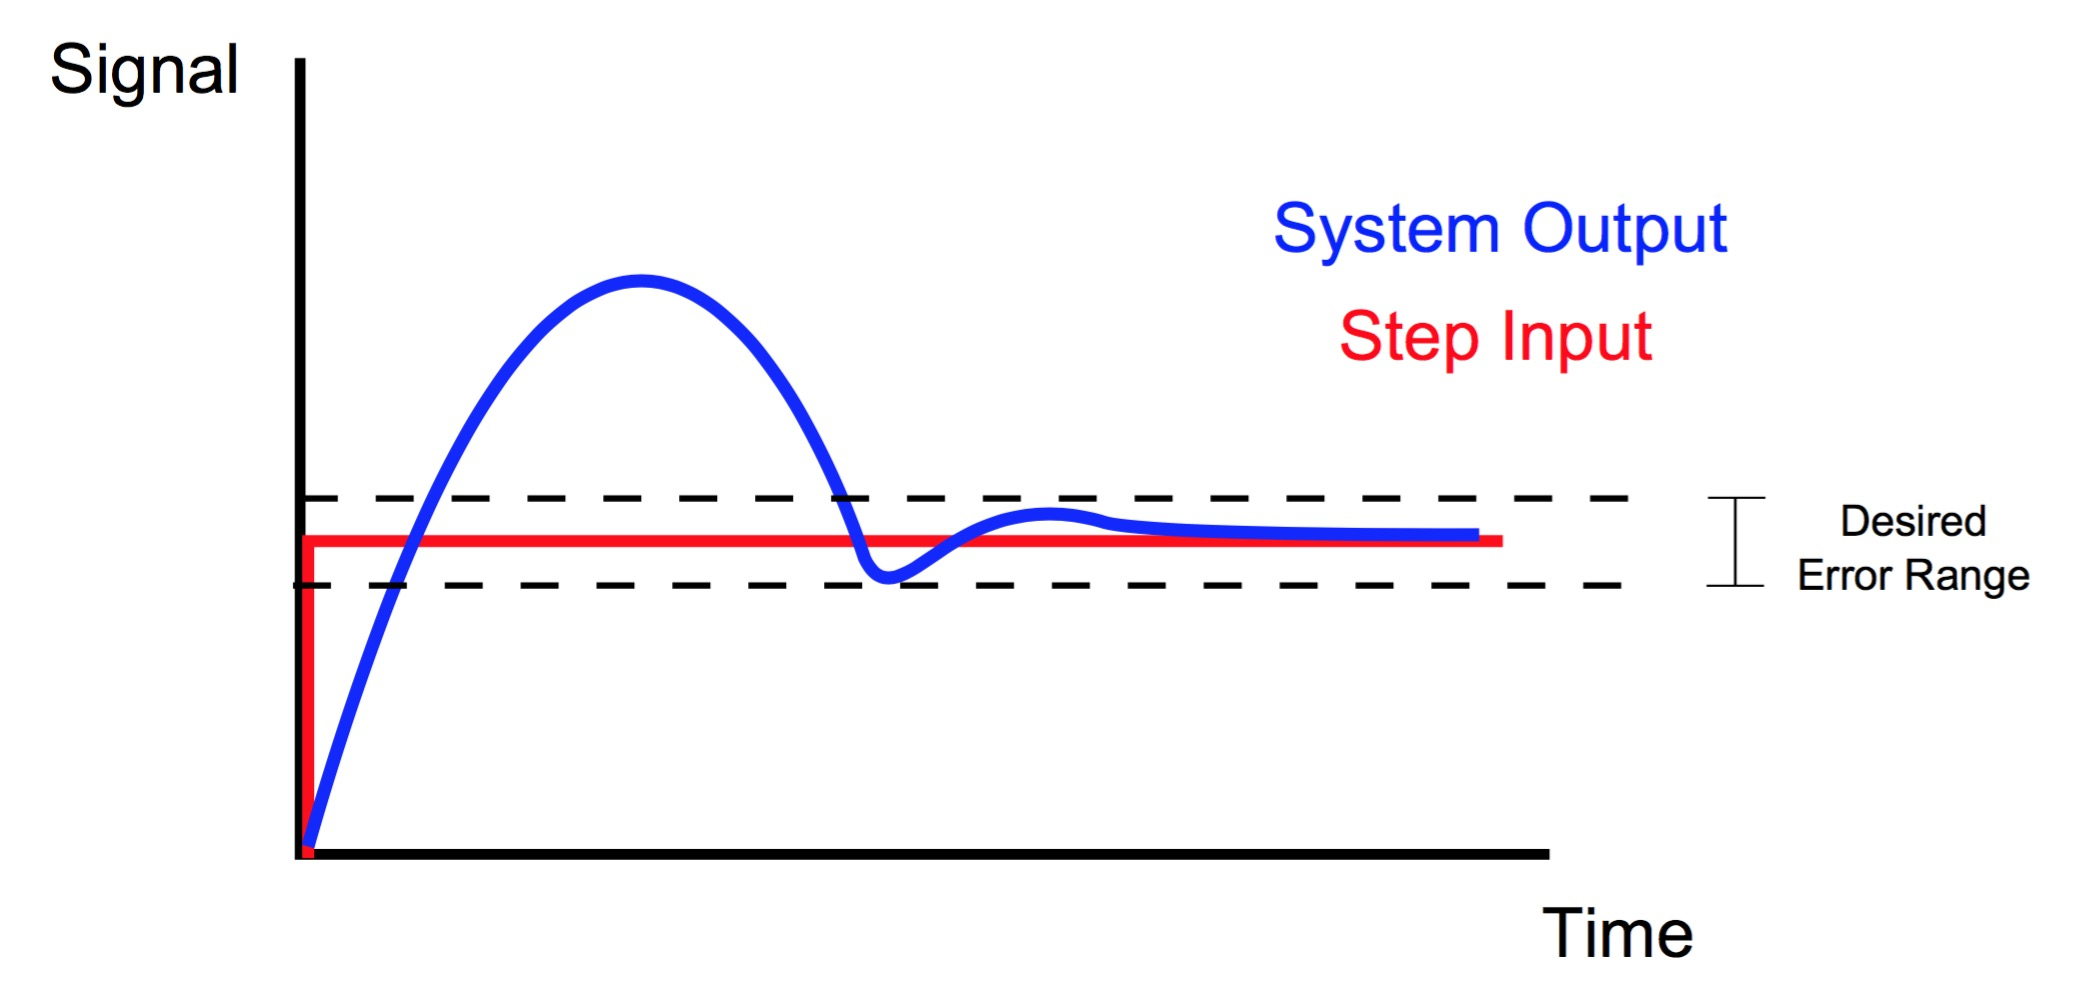
\includegraphics[width=\linewidth]{stable_system.JPG} 
   \caption{Example of Stable System}
   \label{fig:example}
\end{figure}

\bigskip

\addcontentsline{toc}{section}{Procedure \& Analysis} % Add before each section
\section*{\fontsize{12}{12}\selectfont \large Procedure \& Analysis}
The first part of the lab was to obtain the time response of the two given systems. To do so, the systems were first modeled in Simulink, as shown in Figure 3. MATALB was then used to obtain the time response to these systems. The time response to the first (top) system is shown in Figure 4, and the time response to the second (bottom) system is shown in Figure 5. A MATLAB script was also written to calculate the percent overshoot of the systems. As can be seen, the first system is unstable because it does not approach a steady state value; therefore, the first system has quantifiable percent overshoot as indicated after running the MATLAB script, the results of which are shown in Figure 6. It can be seen that the second system is stable because it reaches  a steady state value. The system is calculated by the script to have a percent overshoot of about 25.4\%. The percent overshoot can also be calculated by analyzing the plot and using Equation 3, which results in a percent overshoot of about 25\%.
\bigskip

Another system was then described by only its transfer function, shown in Equation 4, in the second part of the lab. The transfer function was then analyzed using a MATLAB script in order to obtain various system characteristics. The characteristics obtained after running the MATLAB script are shown in Figure 7 and the plot of the system time response is shown in Figure 8. The system was calculated by the MATLAB script to have a percent overshoot of about 10.8\%, while the percent overshoot determined by analyzing the plot  and using Equation 3 was found to be about 11.8\%. The rise time of the system was found to be 0.3121 seconds. The settling time was found to be 1.0213 seconds. This tells us that it took the system barely over 1 second to come to a steady state after being exposed to an external disturbance, in this case a step input. By analyzing the plot of the time response in Figure 8, the steady state value is seen to be around 3.6.
\bigskip
\bigskip

\begin{equation}
TF = \frac{360}{3s^2+20s+100}
\end{equation}

\newpage

\bigskip
\bigskip

% Figure 3
\begin{figure}[h!] %  figure placement: here, top, bottom, or page
   \centering
   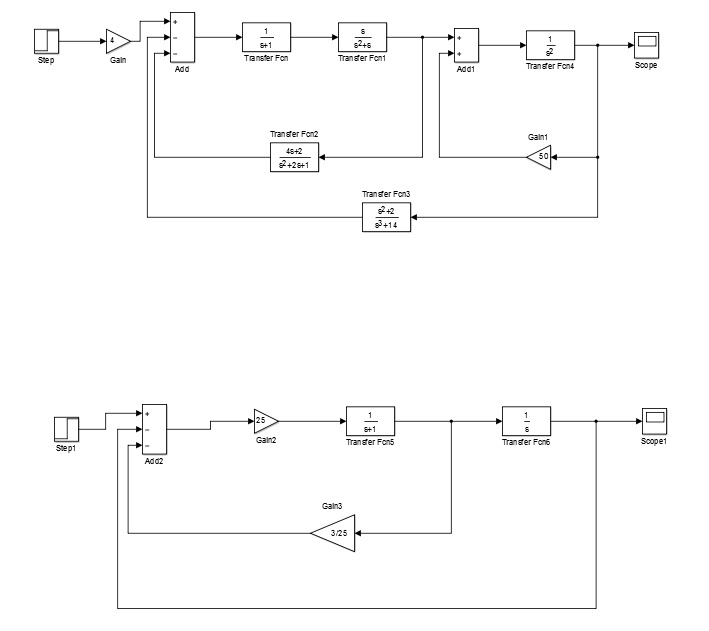
\includegraphics[width=\linewidth,height=7in]{simulink_models.jpg} 
   \caption{Simulink Models}
   \label{fig:example}
\end{figure}

\newpage

% Figure 4
\begin{figure}[h!] %  figure placement: here, top, bottom, or page
   \centering
   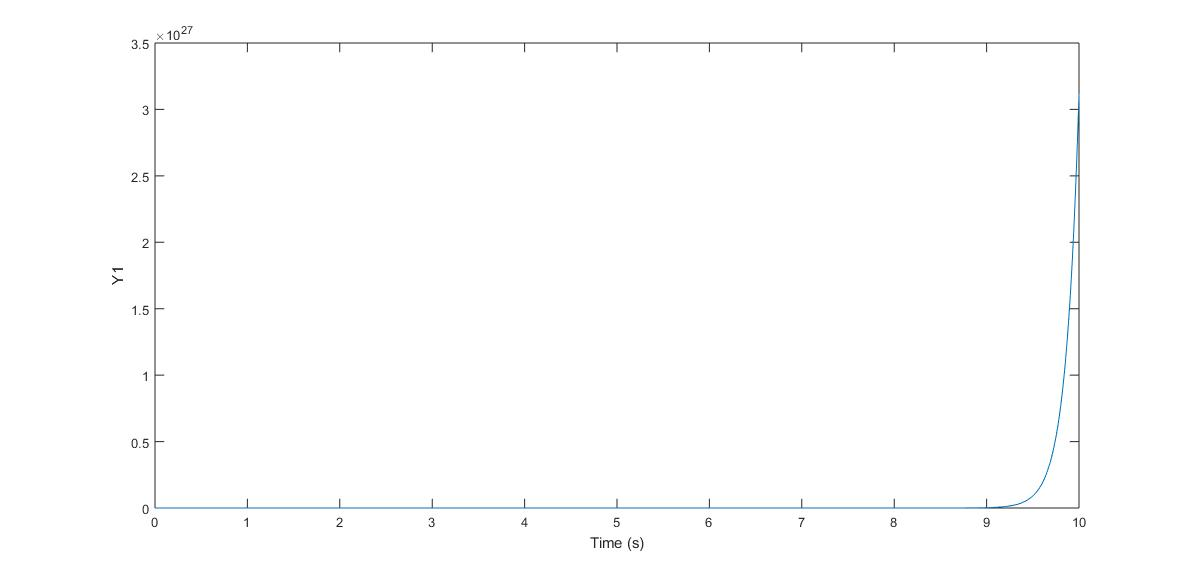
\includegraphics[width=\linewidth]{time_response_system_1.jpg} 
   \caption{Lab Part 1 System 1 Time Response}
   \label{fig:example}
\end{figure}

% Figure 5
\begin{figure}[h!] %  figure placement: here, top, bottom, or page
   \centering
   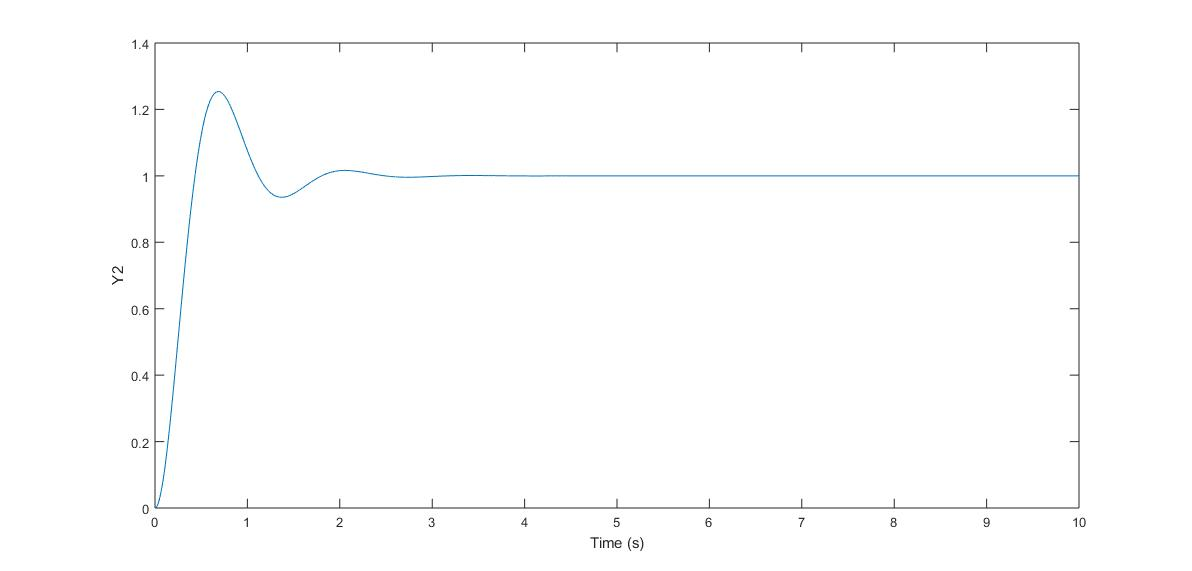
\includegraphics[width=\linewidth]{time_response_system_2.jpg} 
   \caption{Lab Part 1 System 2 Time Response}
   \label{fig:example}
\end{figure}
\bigskip

\newpage

% Figure 6
\begin{figure}[h!] %  figure placement: here, top, bottom, or page
   \centering
   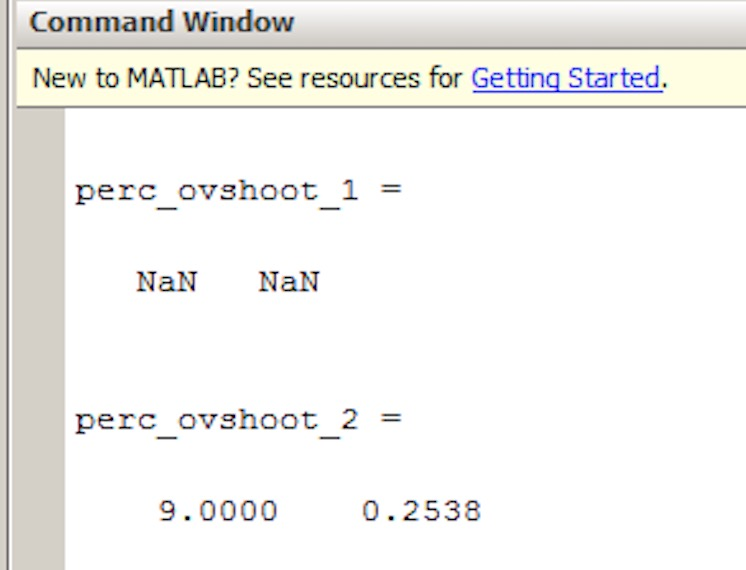
\includegraphics[width=2.5in]{part_1_commandline.jpg} 
   \caption{Lab Part 1 Commandline}
   \label{fig:example}
\end{figure}
\bigskip
\bigskip

% Figure 7
\begin{figure}[h!] %  figure placement: here, top, bottom, or page
   \centering
   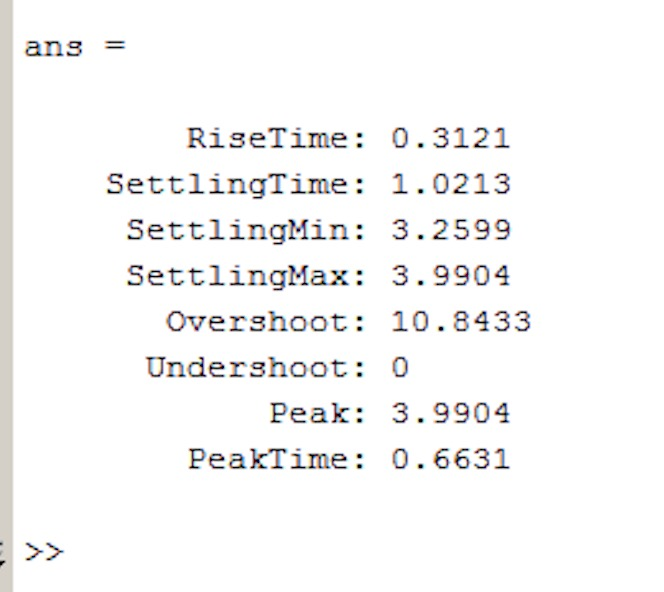
\includegraphics[width=4in]{part_2_commandline.jpg} 
   \caption{Lab Part 2 Commandline}
   \label{fig:example}
\end{figure}

\newpage

% Figure 8
\begin{figure}[h!] %  figure placement: here, top, bottom, or page
   \centering
   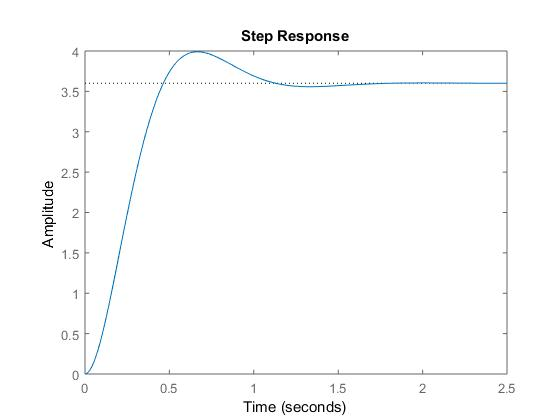
\includegraphics[width=\linewidth]{part_2_time_response.jpg} 
   \caption{Lab Part 2 Time Response}
   \label{fig:example}
\end{figure}
\bigskip



\addcontentsline{toc}{section}{Conclusion} % Add before each section
\section*{\fontsize{12}{12}\selectfont \large Conclusion}
The exercises conducted in the lab reinforce the theory learned in the classroom. It is shown that systems can be modeled and analyzed using MATLAB and Simulink in order to achieve the same system characteristics that can be calculated using various methods and equations. The systems analyzed supplemented firsthand experience with systems in which signals are passed through gains, transfer functions, feedback loops, and summation points. These types of devices are commonplace in modern circuits and control systems, which makes it important to have firsthand experience with them.



%\section*{\fontsize{12}{12}\selectfont \large References}

\begin{thebibliography}{2}

% Example
%\bibitem{Wagner}
%Ng, K., Wagner, S.W., Camelio, J., Emblom, W.J. (2010). ?Experimental Analysis of Micro Tube
%Hydroforming Process.? Transactions of NAMRC of SME, 38, 577-584.

\end{thebibliography}



%\section*{\fontsize{12}{12}\selectfont APPENDIX}

%\begin{table}[h!]
%  \caption{}
%  \includegraphics[width=\linewidth]{table1.png}
%\end{table}




\end{document}







----------------------------Templates-------------------------------

-------------------------Figure-----------------------

\begin{figure}[h!]  
  \centering
    \includegraphics[width=\linewidth]{**file**}
    \caption{Docking Station}
\end{figure}

---------------------------Table-----------------------
\begin{table}[ht]
\caption{Nonlinear Model Results} % title of Table
\centering % used for centering table
\begin{tabular}{c c c c} % centered columns (4 columns)
\hline\hline %inserts double horizontal lines
Case & Method\#1 & Method\#2 & Method\#3 \\ [0.5ex] % inserts table
%heading
\hline % inserts single horizontal line
1 & 50 & 837 & 970 \\ % inserting body of the table
2 & 47 & 877 & 230 \\
3 & 31 & 25 & 415 \\
4 & 35 & 144 & 2356 \\
5 & 45 & 300 & 556 \\ [1ex] % [1ex] adds vertical space
\hline %inserts single line
\end{tabular}
\label{table:nonlin} % is used to refer this table in the text
\end{table}



probably best to insert as an image from excel

\bigskip\\
\begin{table}[h!]
  \caption{}
  \includegraphics[width=\linewidth]{**file**}
\end{table}
\bigskip\\





-----------------------------Equations------------------------
-----------------------------Regular
\begin{equation}
a = b + c
\end{equation}

--------------------------------- Multiline
\begin{multline}
a = b + c + d + e + f
+ g + h + i + j \\
+ k + l + m + n + o
\end{multline}

-------------------------------Citations-------------------------
\bibitem{Author last name}
  Last, First., year of publication,
  article name, book(etc) name, from \\
  link goes here

----------------------------------other-----------------------------

equations:
http://moser-isi.ethz.ch/docs/typeset_equations.pdf

citations:
http://library.missouri.edu/engineering/about/guides/asme
https://www.asme.org/shop/proceedings/conference-publications/references